\documentclass[10pt,journal,compsoc]{IEEEtran}

\ifCLASSOPTIONcompsoc
  \usepackage[nocompress]{cite}
\else
  \usepackage{cite}
\fi

\usepackage{graphicx}  
\usepackage{subfig}
\usepackage{xcolor}

\newcommand\MYhyperrefoptions{bookmarks=true,bookmarksnumbered=true,
pdfpagemode={UseOutlines},plainpages=false,pdfpagelabels=true,
colorlinks=true,linkcolor={black},citecolor={black},urlcolor={black},
pdftitle={Bully and Ring Election Algorithms Performance Analysis Considering
Real Case Aspects},
pdfsubject={Typesetting},
pdfauthor={Michael D. Shell},
pdfkeywords={Computer Society, IEEEtran, journal, LaTeX, paper,
             template}}

\hyphenation{op-tical net-works semi-conduc-tor}

\begin{document}

\title{Bully and Ring Election Algorithms Performance Analysis Considering Real
Case Aspects}

\author{Denise~Comincioli,
        Alessandra~Dalla~Verde}
        
\IEEEtitleabstractindextext{%
    \begin{abstract}
    In the distributed systems field, various papers compared the performance of
    modified classic election algorithms with their original counterpart, by
    using their computational complexity to represent the number of messages
    exchanged. Currently, there is no analysis of classic algorithms'
    simulations, conducted under their theoretical assumptions or in real case
    scenarios. Hence, we decided to simulate the Ring and Bully election
    algorithms in the presence of communication delays and unreliable
    links. We compare their turnaround time and explore how its value changes in
    relation to a series of different factors (e.g. number of nodes). Finally,
    we analyze advantages and disadvantages of deploying the Bully and the Ring
    algorithm, before concluding that application requirements and network
    capabilities determine which one is the best for the distributed system at
    hand.
    \end{abstract}

\begin{IEEEkeywords}
    Election, simulation, performance evaluation, distributed algorithms,
    link failures
\end{IEEEkeywords}}

\maketitle

\IEEEdisplaynontitleabstractindextext
\IEEEpeerreviewmaketitle

\ifCLASSOPTIONcompsoc
\IEEEraisesectionheading{\section{Introduction}\label{sec:introduction}}
\else
\section{Introduction}
\label{sec:introduction}
\fi

\IEEEPARstart{I}{n} a distributed system having a coordinator node to manage
operations is common practice. When the coordinator becomes unavailable or
crashes, a new one must be selected to keep the system operating. This is
achieved by using election algorithms, which guarantee consensus of all active
processes on the new coordinator. 
\\The Bully \cite{paper:bully} and the Ring algorithm  \cite{paper:ring} are
two classic election procedures. They have strong assumptions difficult to
satisfy in a real system, where failures may occur and communication delays are
a certainty. This paper aims to compare their performance based on turnaround
times \footnote{The terms turnaround time and runtime are used interchangeably
throughout this paper.}, exposing critical issues that may arise when breaking
one or more assumptions. 
\\In the following sections, we discuss: constraints and implementation choices,
simulation core concepts, the performance analysis process and the most
interesting simulations' final results.
%-------------------------------------
%-------------------------------------
%-------------------------------------
\section{Assumptions}
\label{sec:assumptions}
The constraints we set for the Bully and Ring algorithms are extracted from
academic literature and combined with some additional conditions. This
integration was done to simplify implementation and allow for a better, fairer
comparison of the two algorithms. 
\\To build our set of assumptions, we referred to: the \emph{Elections in a
Distributed Computing System} paper by Garcia-Molina\cite{paper:bully} for the
Bully Algorithm, and the \emph{Distributed Systems} book by van Steen and
Tanenbaum\cite{book:ds}, containing a simplification of Chang and Roberts'
original work \cite{paper:ring}, for the Ring Algorithm. To summarize, we list
our main assumptions for the final system:
\begin{itemize}
    \item Distinguishable nodes: each node has a unique ID; IDs follow a total
    order.
    \item Closed system: nodes know all their peers; no processes can leave or
    enter the network.
    \item Asynchronous system.
    \item Reliable nodes: aside from the initial coordinator crash, no other
    node can fail during the election.
    \item Fully connected topology: every node is directly connected to all
    others.
\end{itemize}
According to the literature, the Ring algorithm requires nodes to be arranged
in a logical ring, i.e., an overlay network. Nevertheless, we included the last
point to allow more flexibility and achieve a common network architecture for
both algorithms. This topology change does not impact the Ring algorithm's
performance, as the nodes are still organized in a virtual ring based on their
IDs.
\\Before proceeding with the implementation choices, we delve into the nature of
the networks links we considered and the asynchronicity assumption.
%-------------------------------------
%-------------------------------------
\subsection{Reliable and Unreliable Links}
\label{sec:unreliable}
In the literature, the original formulation of the algorithms required the links
to be reliable, meaning all messages were assumed to always arrive to the
intended destination correct.
In a real system, reliable links are expensive and difficult to achieve:
different types of failures have to be managed, ranging from transmission errors
to packet losses. Hence, we decided to analyze how the Ring and Bully algorithms
performed when accounting for packet loss, in addition to measuring how they
fared in the reliable case. When testing with unreliable links, both algorithms
require the system to be synchronous. 
%-------------------------------------
%-------------------------------------
\subsection{Asynchronicity}
\label{sec:asyn}
An asynchronous distributed system allows no assumptions about message
propagation delays, clock drift rates and process execution speeds
\cite{book:ds_c_and_d}. 
Following this definition, the Bully algorithm breaks in an asynchronous system.
A node becomes the new coordinator only when peers with a higher ID do not
respond to the election messages it sent. This means that a process cannot
simply wait for a response for an unbounded amount of time, as it might never
receive one. Every node would need to know exactly the maximum round-trip-time
to ensure the algorithm eventually terminates and is correct.
\\We minimized the issue by setting a maximum wait time that could cover the
majority of the network delays generated. As a consequence, the performance of
the Bully algorithm worsens, i.e., the turnaround time increases. Nevertheless,
we can still collect valuable data from these simulations.
The Ring algorithm under the reliable links assumption, does not present the
same problem.
\\On the other hand, as discussed in Section \ref{sec:unreliable}, when
considering unreliable links both procedures require a synchronous system. This
stems from the fact that nodes need to distinguish lost from slow messages.
Setting maximum timeouts is the easiest solution, as mistakenly retransmitting a
slow message does not effect the outcome of the election process. We further
cover this topic in Section \ref{sec:delays}.
%-------------------------------------
%-------------------------------------
%-------------------------------------
\section{Implementation Choices}
\label{sec:implementation}
This section explains how we implemented the two algorithms under the
assumptions of reliable and unreliable links. In addition, it lists the factors
that may influence the simulations' results and explains how we set them.
%-------------------------------------
%-------------------------------------
\subsection{Algorithms Implementation}
\label{sec:implementation}
The Bully and the Ring algorithm rely on SimPy, "a process-based discrete-event
simulation framework based on standard Python"\cite{book:simpy}, which allows us
to manage process concurrency without threads, locks, or other low-level
constructs. We chose to use this library to focus more on the implementation of
the two algorithms.
\\In SimPy time is unitless, but developers can decide to give it the unit of
measurement they prefer, as described in Section 3.2.2 of the SimPy
documentation \cite{book:simpytime}. For this project we chose to use
milliseconds, therefore, the performance results are expressed in this unit.
%-------------------------------------
%-------------------------------------
\subsection{Unreliable Links Implementation}
\label{sec:unrel_implementation}
Aside from the alterations already discussed in Section \ref{sec:asyn}, we had
to implement more robust versions of the original algorithms to handle
unreliable links. We integrated a fault tolerance technique to guarantee
termination and, for the Bully algorithm only, correctness. In particular,
we chose to adopt the retransmission strategy. It works as follows: a node sends
a message, sets a timeout and waits for the acknowledgment from the receiver.
If the ACK does not arrive before the timeout, the original sender retransmits
the packet. ACKs can be lost, but the election final result remains correct even
if a node receives a duplicated message. Performance-wise, this strategy causes
the number of messages sent to increase for both the Bully and Ring algorithm.
\\In our simulation, packets are considered as lost if a randomly generated
number ranging from 0 to 1 is lesser or equal than a loss rate parameter.
%-------------------------------------
%-------------------------------------
\subsection{Initiators}
The original Ring and Bully algorithms accept a variable number of initiators,
i.e., nodes which detect the coordinator's crash and start the election. We
decided to keep this feature for all the algorithms' versions.
%-------------------------------------
%-------------------------------------
\subsection{Delays and Timeouts}
\label{sec:delays}
To simulate more realistic scenarios, we decided to generate random message
delays. The paper \emph{A Probabilistic Approach to Distributed Clock
Synchronization} by Flaviu \cite{paper:delays} addresses the issue of
unpredictable communication delays in distributed systems and models them
following a log-normal distribution. Therefore, in our system, we adopted a
distribution with a similar trend for delay generation: the exponential. We
chose it as it allowed for easier data extrapolation given its dependency on
only one parameter, the rate, instead of two, like in the log-normal case.
\\In our algorithms, timeouts are set based on the maximum message delay
possible to avoid breaking the election procedure. However, given the
exponential distribution of the delays, arbitrarily large values can be
generated, even if with low probability, meaning there is not a real maximum
wait time. Hence, we computed timeouts based on a quantile parameter. 
\\As discussed in Section \ref{sec:asyn}, the Bully algorithm under the reliable
links assumption requires timeouts to guarantee that eventually the active node
with highest ID will be elected as the new coordinator. Regardless of the
timeout value we set, the probability of a node missing a slow response and
causing the wrong process to be elected, cannot be reduced to zero. Therefore,
when testing under these assumptions, we set the quantile parameter to 0.99,
which guarantees that more than 99\% of the simulations ran are correct, as seen
in \emph{figure \ref{fig:wrg_a}}. The consequence of choosing higher quantile
values is highlighted by \emph{figure \ref{fig:wrg_b}}, where we can observe an
increase of the election turnaround time.
\\To collect the data shown in \emph{figure \ref{fig:wrg}}, we ran the Bully
algorithm 1000 times, counted the number of invalid simulations and stored the
mean turnaround time. We then repeated this process 500 times for each quantile.
In this case, we used a simulation environment with the following parameters:
network size of 5 nodes, 1 election initiator and a delay mean of 110 ms. 
\\When considering unreliable links, we set for both algorithms a quantile
parameter of 0.8, as the retransmission of messages prevents these type of
issues.
\begin{figure}[t!]
    \centering
    \subfloat[Percentage of Wrong Simulations\label{fig:wrg_a}]
    {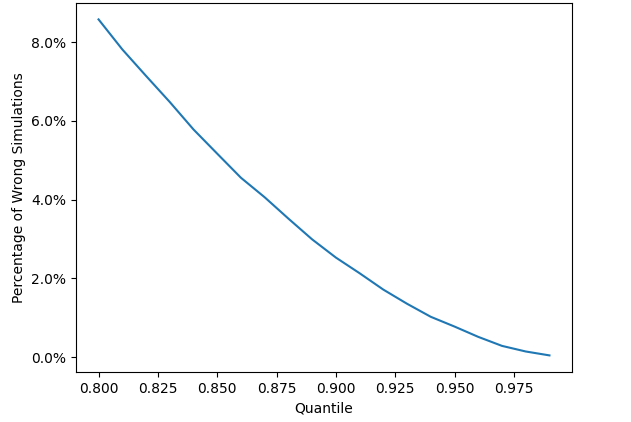
\includegraphics[width=0.3\textwidth]{figs/wrg_sim.png}}
    \hfil
    \subfloat[Turnaround Time\label{fig:wrg_b}]
    {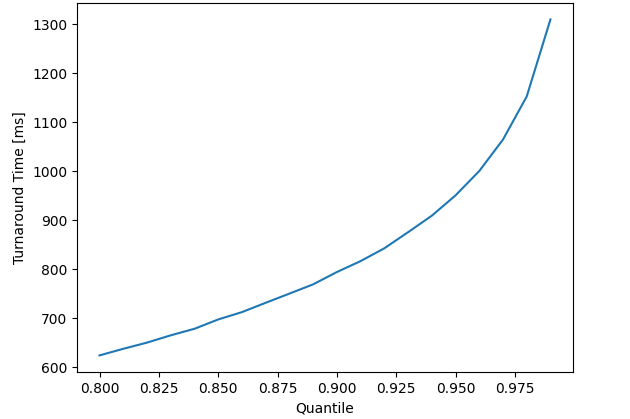
\includegraphics[width=0.3\textwidth]{figs/wrg_sim_runtime.png}}
    \caption{Exponential Quantile Analysis of Reliable Bully Algorithm}
    \label{fig:wrg}
\end{figure}
%-------------------------------------
%-------------------------------------
\subsection{Number of Nodes}
\label{sec:nodes}
"Many leader election algorithms apply to only relatively small distributed
systems" \cite{book:nodes}. To verify that this statement holds also for the
Bully and Ring algorithms, we performed simulations with the same parameters on
networks of different size, where the number of nodes ranged from 3 to 25. 
\\We set the other environment parameters, i.e., number of initiators and delay
mean, equal to the ones used to collect data for the quantile graphs of Section 
\ref{sec:delays}. For each type of simulation, we run the two algorithms 10000
times, storing the mean of the turnaround time and the mean of the number of
messages. 
Based on these metrics, we can observe that the performance of the two
algorithms decreases as the number of nodes grows, which is highlighted by
\emph{figure \ref{fig:n_nodes}}. In particular,
\emph{figure \ref{fig:n_nodes_a}} shows that the number of messages and the
turnaround time of the Ring algorithm increase linearly with the number of
nodes. The number of messages may be affordable, but not the turnaround time.
Meanwhile, we can see from \emph{figure \ref{fig:n_nodes_b}} that the Bully
algorithm runtime grows slower, but the number of messages increases rapidly. If
a distributed system needs to avoid traffic caused by only control messages,
this last algorithm is not recommended. A similar argument can be made with the
versions of both procedures for the unreliable links assumption and is provided
in the Appendix (see \emph{figure \ref{fig:n_nodes_unreliable}}).
\\Based on the results presented, we decided to simulate the two algorithms with
small networks.
\begin{figure}[t!]
    \centering
    \subfloat[\label{fig:n_nodes_a}]{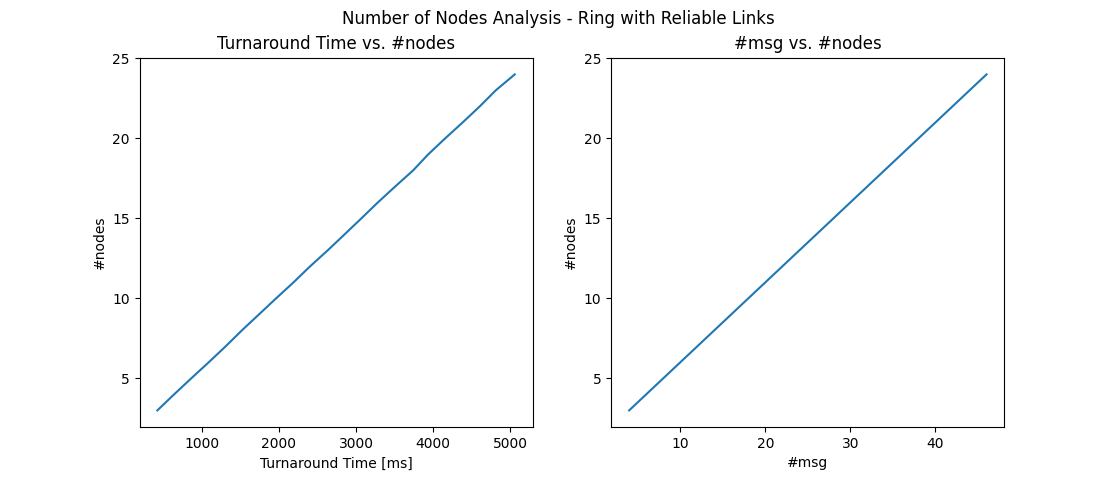
\includegraphics[width=0.45\textwidth]
    {figs/n_nodes_ring.png}}
    \hfil
    \subfloat[\label{fig:n_nodes_b}]{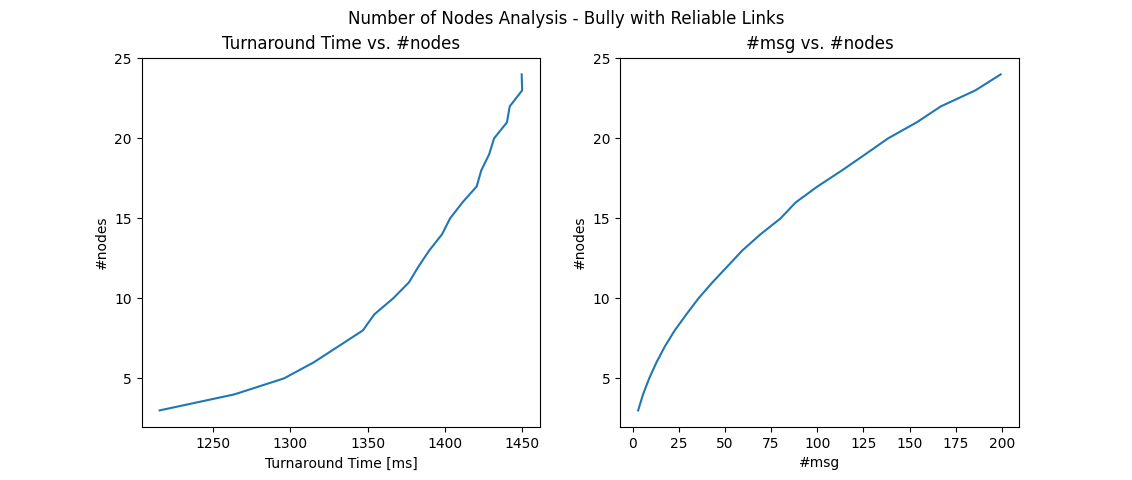
\includegraphics[width=0.45\textwidth]
    {figs/n_nodes_bully.png}}
    \caption{Number of Nodes vs. Number of Messages and Turnaround Time}
    \label{fig:n_nodes}
\end{figure}
%-------------------------------------
%-------------------------------------
%-------------------------------------
\section{Performance Analysis}
We evaluated the performance of the two election algorithms based on two
metrics: the number of messages sent and the turnaround time, i.e., the time the
network takes to reach consensus on the new coordinator.
\\We created different testing scenarios by changing the following parameters:
number of nodes, loss rate and number of initiators. We kept the mean of the
exponential delay distribution fixed at 110 ms.\\
In total we tested networks with 4, 5, 6 and 8 nodes in scenarios with: 20\%,
50\% or 75\% loss rate, and 1, 3 or 4 election initiators.
For convenience, in later sections we use the words "\textit{default scenario}"
to refer to cases in which: the network has 5 nodes, there is only one initiator
and, if under the unreliable link assumption, the loss rate is set to 20\%. 
\\We computed the two performance metrics by applying the same procedure used in
Sections \ref{sec:delays} and \ref{sec:nodes}: to achieve reliable data, we
repeated the execution of each algorithm 10000 times. We decided to exclude the
outliers by following the IQR method, before computing the sample variance, the
sample mean, and the mean 95\%-confidence interval. 
%-------------------------------------
%-------------------------------------
%-------------------------------------
\section{Results}
This section shows the results we achieved from the simulations. First, we
analyze the performance of the two algorithms separately, then we compare them.
%-------------------------------------
%-------------------------------------
\subsection{Bully Algorithm Analysis}
\label{sec:bully_general_analysis}
Before proceeding with version-specific observations, we offer some insights on
behaviors shared by both the reliable and unreliable links versions of the Bully
algorithm. As expected, a higher number of nodes causes an increase of both the
turnaround time and the number of messages. Additionally, in similar
simulations, a higher initiator count corresponds to a runtime decrease and a
message increase. The latter phenomenon is explained by the fact that, even if
later interrupted, at least in the beginning each initiator separately starts
their own election. On the other hand, the algorithm turnaround time improves
because the more initiators are involved, the higher are the chances to produce
an election where the number of nodes to contact and the generated delays are
lower. Essentially, the fastest conducted election eventually suppresses all
others.     
\begin{figure}[t!]
    \centering
    \subfloat[\label{fig:bully_a}]{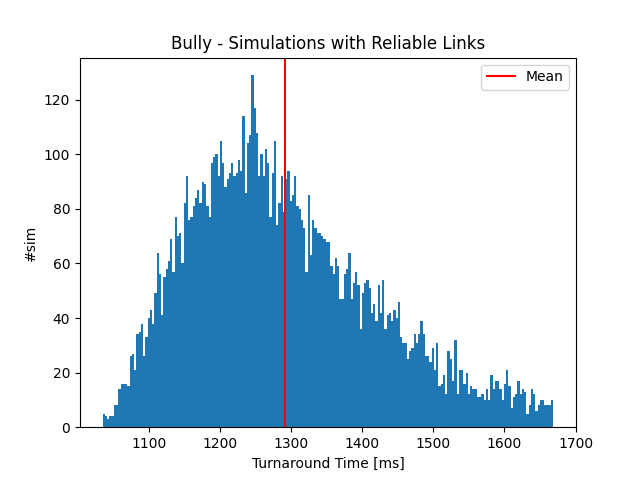
\includegraphics[width=0.3\textwidth]
    {figs/bully_hist.png}}
    \hfil
    \subfloat[\label{fig:bully_b}]{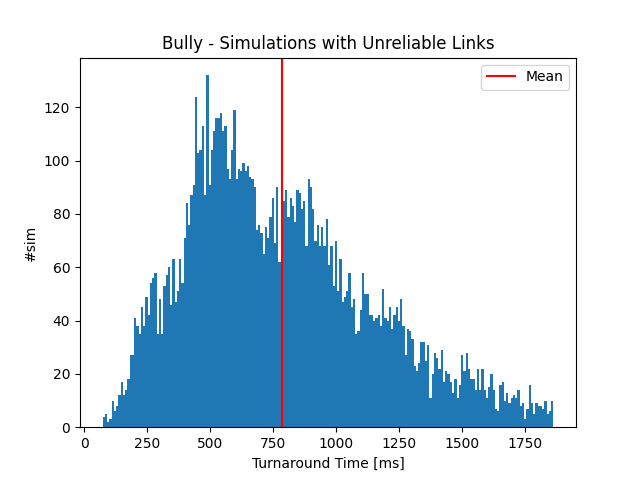
\includegraphics[width=0.3\textwidth]
    {figs/bully_hist_unreliable.png}}
    \caption{Bully Algorithm Turnaround Time Analysis}
\end{figure}
\begin{figure}
\centering
        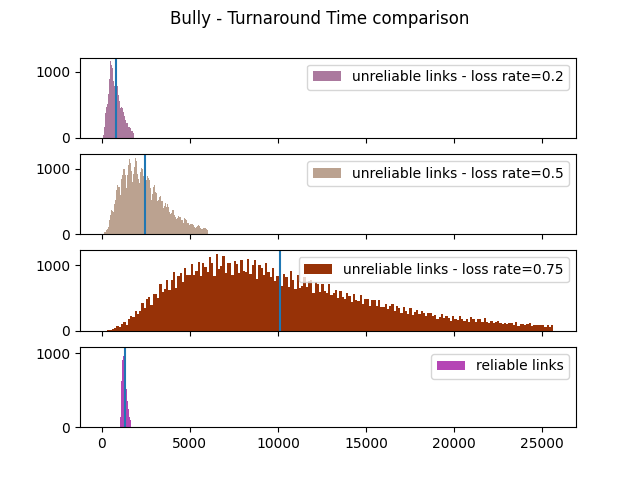
\includegraphics[width=0.4\textwidth]{figs/bully_compare.png}
    \caption{Bully Algorithm Turnaround Time Comparison with Reliable and
    Unreliable links}
    \label{fig:bully_c}
\end{figure}
%-------------------------------------
\subsubsection{Reliable Links}
\label{sec:bully_reliable}
When considering the \textit{default scenario}, under the reliable links
assumption, the Bully algorithm has a mean turnaround time of 1290.83 ± 2.61 ms
and a 17234.51 ms\textsuperscript{2} variance. As previously discussed, the
quantile parameter was set to 0.99. The presence of high variance in the data is
explained by the random choice of the initiator: if the starting node is already
the one with highest ID, the election terminates almost immediately, while if it
has the lowest ID and the generated message delays are particularly high, the
procedure will take longer.\\In \textit{figure \ref{fig:bully_a}}, we can see
that the turnaround time distribution skews to the left, indicating that it is
more common for the algorithm to have lower runtimes. 
\subsubsection{Unreliable Links}
\label{sec:bully_unreliable}
In the \textit{default scenario} under the unreliable links assumption, the
Bully algorithm has a mean turnaround time of 786.02 ± 7.38 ms and a 137489.76
ms\textsuperscript{2} variance. \\Against expectations, it might appear that the
algorithm performs better with unreliable links, but it is not as it seems. We
already highlighted in Section \ref{sec:delays} that the quantile parameter used
for this case is 0.8, therefore all maximum wait times are reduced compared to
the reliable version of the algorithm. 
Only when the number of messages lost is relatively low, i.e., when the loss
rate is less than approximately 45\%, the reduced wait times can offset the cost
of retransmitting packets. When the loss rate exceeds 45\%, the Bully algorithm
performs worse when under the unreliable links assumption. We can see this
phenomenon in \textit{figure \ref{fig:bully_c}}.
%-------------------------------------
%-------------------------------------
\subsection{Ring Algorithm Analysis}
The general considerations made in Section \ref{sec:bully_general_analysis} are
also valid for the Ring algorithm: the turnaround time decreases as the number
of initiators increases. The Ring algorithm stops when an initiator receives
back their message after it completed two round trips of the ring. Hence,
smaller communication delays cause the election started by one initiator to win
over the others, affecting the final turnaround time and increasing the number
of messages sent.
%-------------------------------------
\subsubsection{Reliable Links}
The reliable Ring algorithm, in the \textit{default scenario}, has a turnaround
time mean of 862.88 ± 5.68 ms and a turnaround time variance of 82618.75
ms\textsuperscript{2}. 
\\As in the case of the reliable Bully algorithm, the variance is very high,
but it is only attributed to the randomization of the exponential delays. Due to
the fact that messages are exchanged only between two neighbors, and the
election does not proceed before the receiver has processed the message, the
performance of the algorithm is strictly influenced by how much time a message
takes to be transmitted. 
\\In \textit{figure \ref{fig:ring_a}} we present the histogram of the reliable
Ring algorithm turnaround time in the \textit{default scenario}. It behaves like
a Gamma distribution, as we are summing 10000 Gamma-distributed samples, each
obtained as the sum of random exponential sample values. 
\begin{figure}[t!]
    \centering
    \subfloat[\label{fig:ring_a}]{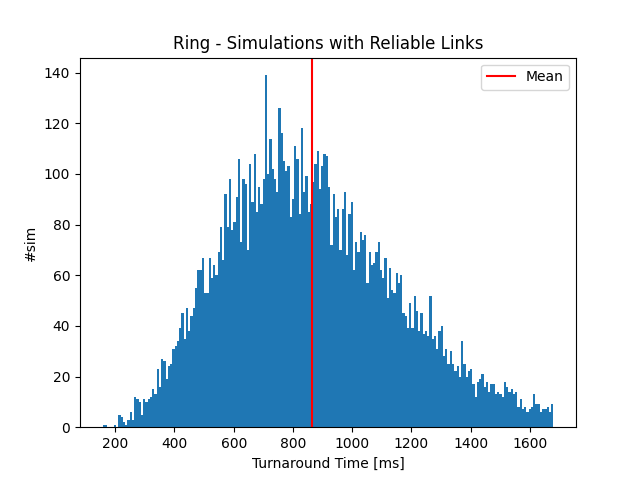
\includegraphics[width=0.3\textwidth]
    {figs/ring_hist.png}}
    \hfil
    \subfloat[\label{fig:ring_b}]{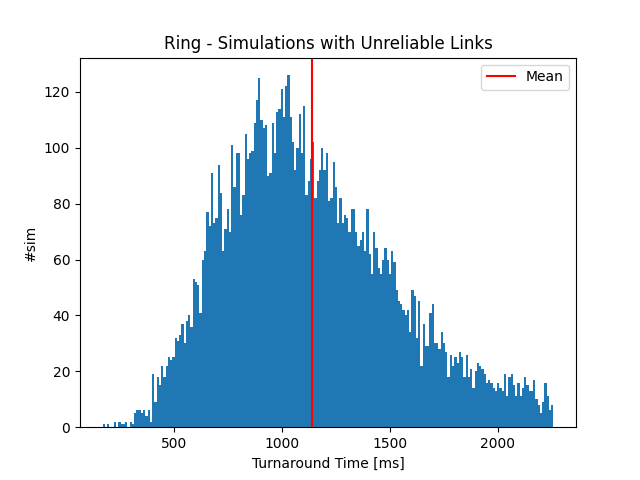
\includegraphics[width=0.3\textwidth]
    {figs/ring_hist_unreliable.png}}
    \caption{Ring Algorithm Turnaround Time Analysis}
    \label{fig:ring}
\end{figure}
%-------------------------------------
\subsubsection{Unreliable Links}
The Ring algorithm with unreliable links, in the \textit{default scenario}, has
a turnaround time mean of 1137.66 ± 7.84 ms and a turnaround time variance of
156166.45 ms\textsuperscript{2}. Compared to the reliable links version, the
performance worsens due to packets loss. The considerations we made about the
distribution in the previous section also hold in this case, but we do not have
an exact Gamma distribution, as we see in \emph{figure \ref{fig:ring_b}}. This
is caused by the variability of the number of messages. 
%-------------------------------------
%-------------------------------------
\subsection{Bully and Ring Algorithms Comparison}
%-------------------------------------
\subsubsection{Reliable Links}
In \textit{figure \ref{fig:box_plots}} we show the turnaround time box plots for
the Bully and Ring algorithms with reliable links. The simulations we ran used
the \textit{default scenario} parameters. Due to the quantile set for timeouts,
the Ring algorithm performs better than the Bully. Specifically, the former has
lower turnaround times because it does not rely on timeouts, and therefore is
not penalized by them, as already mentioned in section \ref{sec:bully_reliable}.
We do not show other additional plots, because, even when considering other
testing scenarios, the relation between the Ring and Bully algorithms remains
the same. This changes only when analyzing networks with more than 8 nodes, but
as discussed in Section \ref{sec:nodes}, we are not interested in doing so.

\begin{figure}
\centering
    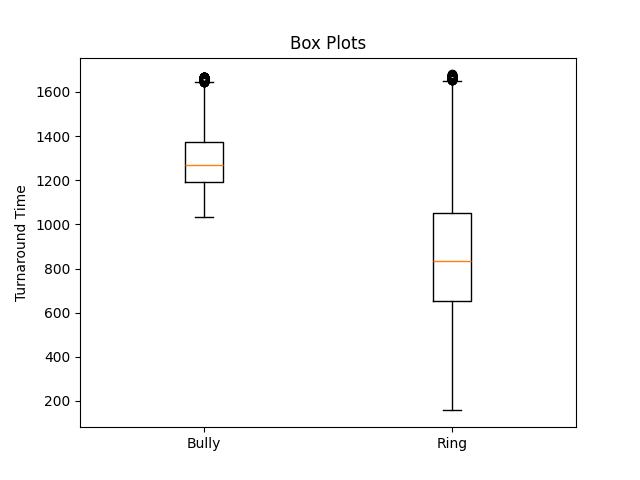
\includegraphics[width=0.3\textwidth]{figs/box_plots.png}
    \caption{Turnaround Time Box Plots of Ring and Bully Algorithms}
    \label{fig:box_plots}
\end{figure}
%-------------------------------------
\subsubsection{Unreliable Links}
With unreliable links, based on the chosen loss rate, the relation between the
Ring and Bully algorithms changes significantly. In the
\textit{default scenario} (\emph{figure \ref{fig:boxplots_a}}), the Bully
algorithm performs better than the Ring. Unlike the reliable case, here the Ring
algorithm is also penalized by timeouts. Furthermore, when a packet is lost
during the Ring election, the messages exchange is stuck between two neighbors.
Until the receiver processes the packet, the transmitter must continue to send
the lost message to the same node. Instead, in the Bully algorithm, multiple
processes can simultaneously send messages to other nodes. Hence, even if some
packets are lost, nodes can receive information from different transmitters.
This ensures a faster election.
\\With loss rates greater than approximately 45\%, the Ring algorithm wins over
the Bully algorithm. \emph{Figure  \ref{fig:boxplots_b}} shows this phenomenon
with a loss rate of 75\%. Packets losses tend to penalize more the Bully
algorithm, as explained in Section \ref{sec:bully_unreliable}.
\begin{figure}[t!]
    \centering
    \subfloat[Loss Rate of 0.2\label{fig:boxplots_a}]
    {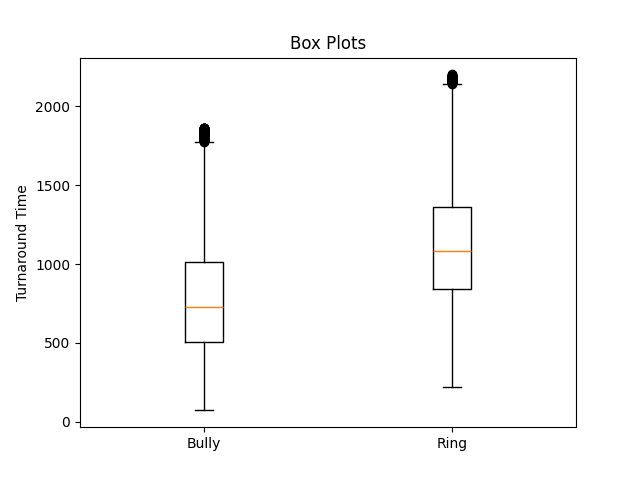
\includegraphics[width=0.3\textwidth]{figs/box_plots_unreliable_1.png}}
    \hfil
    \subfloat[Loss Rate of 0.75\label{fig:boxplots_b}]
    {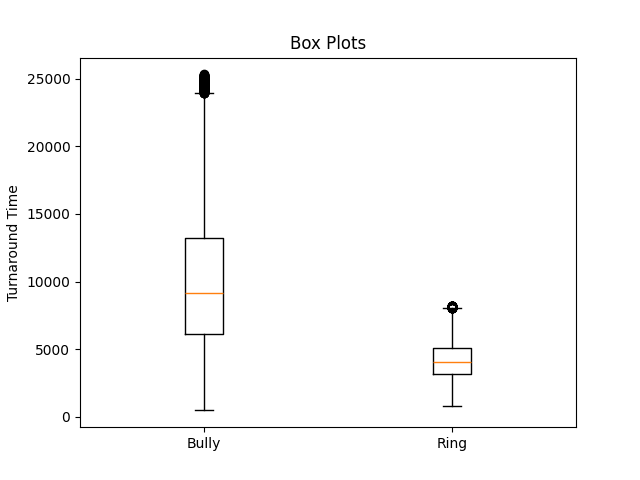
\includegraphics[width=0.3\textwidth]{figs/box_plots_unreliable_2.png}}
    \caption{Turnaround Time Box Plots of Ring and Bully Algorithms with
    Unreliable Links}
\end{figure}
%-------------------------------------
%-------------------------------------
%-------------------------------------
\section{Conclusion}
After conducting our analysis, we can determine that there is no absolute best
performing election algorithm between the two. 
In general, having more initiators decreases turnaround time, but a threshold
should be determined to avoid clogging the channels. 
When considering reliable links, it is clear that applying a Bully algorithm
requires more adjustments due to the costly network assumptions needed to make
it work as intended. Therefore in this case the simplicity of the Ring algorithm
allows for better performance and more predictability. These aspects can be very
valuable to reduce election related traffic in a small distributed system.
Nevertheless, the Ring algorithm has a hidden operational cost related to
maintaining the virtual ring structure when the topology changes.   
In practice, where networks do not normally reach a 45\% loss rate, the
situation is reversed and the unreliable links version of the Bully algorithm
appears to be the best candidate.
To conclude, our paper presented interesting and relevant aspects of applying
two of the simplest election algorithms known. For a more complete evaluation,
our work should be integrated with studies accounting for process failures.

\appendix[Number of Nodes Analysis under Unreliable Links]
As the reliable links case, the performance of the Ring and Bully algorithms
under unreliable links decreases as the number of nodes grows. \emph{Figure 
\ref{fig:n_nodes_unreliable}} shows this result under the same conditions and
with the same procedure described in Section \ref{sec:nodes}. The most relevant
aspect regards the Ring algorithm. Observing the number of messages
(\emph{figure \ref{fig:n_nodes_unreliable_a}}), the control traffic generated is
difficult to manage.
\\Instead, the Bully algorithm with unreliable links (\emph{figure
\ref{fig:n_nodes_unreliable_b}}) is pretty similar to the reliable links case.   
\begin{figure}[!t]
    \centering
    \subfloat[\label{fig:n_nodes_unreliable_a}]
    {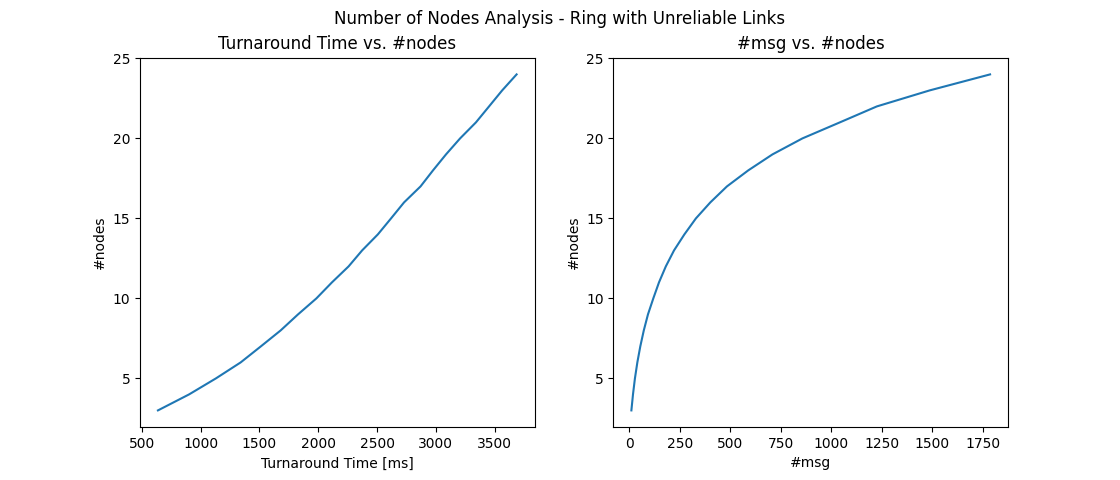
\includegraphics[width=0.45\textwidth]{figs/n_nodes_ring_unreliable.png}}
    \hfil
    \subfloat[\label{fig:n_nodes_unreliable_b}]
    {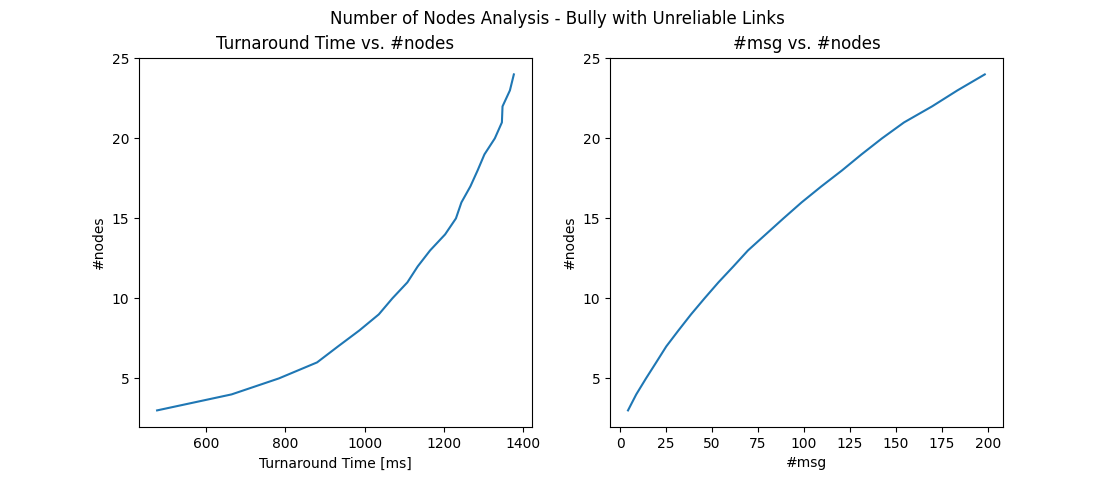
\includegraphics[width=0.45\textwidth]{figs/n_nodes_bully_unreliable.png}}
    \caption{Number of Nodes vs. Number of Messages and Turnaround Time with
    Unreliable Links}
    \label{fig:n_nodes_unreliable}
\end{figure}

\ifCLASSOPTIONcaptionsoff
  \newpage
\fi

\begin{thebibliography}{1}

\bibitem{paper:bully}
H.~Garcia-Molina, \emph{Elections in a Distributed Computing System}, IEEE Tr.
on Comp., Vol. C-31, NO. 1, Jan. 1982.

\bibitem{paper:ring}
E.~J.~H.~Chang and R.~Roberts, \emph{An improved algorithm for decentralized
extremal finding in circular configurations of processes}, Communications of the
ACM, vol. 22, no. 5, pp. 281–283, 1979.

\bibitem{book:ds}
M.~van~Steen and A.~S.~Tanenbaum, \emph{Distributed Systems}, 4th ed., Version
4.03, Jan. 2025, ch. 5, sec. 5.4.2.

\bibitem{book:ds_c_and_d}
G.~Coulouris, J.~Dollimore, T.~Kindberg, and G.~Blair, \emph{Distributed
Systems: Concepts and Design}, 5th ed. Boston, MA: Addison-Wesley, 2012, ch. 2,
sec. 2.4.1.

\bibitem{book:simpy}
Team SimPy, \emph{SimPy Documentation}, Release 4.0.0, Apr. 8, 2020. 

\bibitem{book:simpytime}
Team SimPy, \emph{SimPy Documentation}, Release 4.0.0, Apr. 8, 2020, ch.3,
sec. 3.2.2. 

\bibitem{paper:delays}
F.~Cristian, \emph{A probabilistic approach to distributed clock
synchronization}, in Proc. 9th Int. Conf. Distrib. Comput. Syst., 1989,
pp. 288–296.

\bibitem{book:nodes}
M.~van~Steen and A.~S.~Tanenbaum, \emph{Distributed Systems}, 4th ed., Version
4.03, Jan. 2025, ch. 5, sec. 5.4.5.

\end{thebibliography}

\end{document}